\section{Sistema proposto}
\begin{frame}{Sistema de arquivo distribuído com RAID}
	
	\begin{columns}
		\column{0.5\textwidth}
		\begin{itemize}
			\item Os arquivos são divididos em vários blocos.
			\item Gera a paridade para grupo de alguns blocos.
			\item Armazena distribuidamente por servidores.
			\item Fornece tolerância a falha e distribuição de carga com menos espaço usado por parte redundante.
		\end{itemize}
		\column{0.5\textwidth}
		
		\begin{figure}
			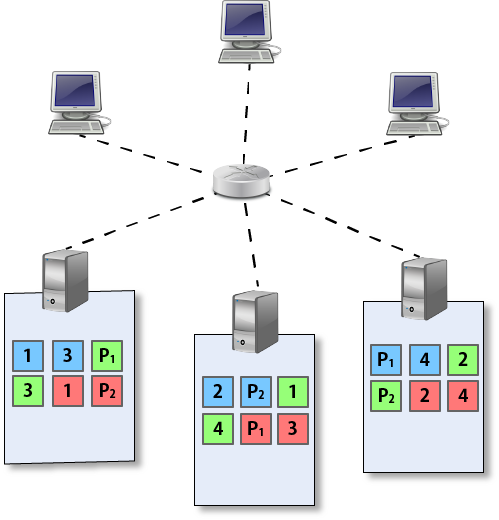
\includegraphics[width=\textwidth]{imagens/image4}
			%\caption{}
			\label{fig:exemplo}
		\end{figure}
	\end{columns}
	
\end{frame}


\begin{frame}{}
	
	\begin{figure}
		\includegraphics[width=\textwidth]{imagens/image5}
		\caption{Geração de paridade e recuperação de arquivo}
		\label{fig:exemplo}
	\end{figure}
	
\end{frame}